
% Lecture Template for FE Exam Review Tristan Hill - Spring 2020 - Fall 2020 - Spring 2021
% FE Exam Revfiew 
% Chapter 7 - Statics
% Lecture 1 - Overview


% Document settings

%\documentclass{beamer}                  % for presentation ?
\documentclass[handout]{beamer}  % for handout ?
\usepackage{beamerthemesplit}
\usepackage{amsmath}
\usepackage{listings}
\usepackage{multicol}
\usepackage{framed}
\usepackage{amsmath, nccmath}
\usepackage{geometry}
\usepackage{bm}

\beamertemplateballitem

\definecolor{TTUpurple}{rgb}{0.3098, 0.1607, 0.5176} % TTU Purple (primary)
\definecolor{TTUgold}{rgb}{1.0000, 0.8666, 0.0000} % TTU Gold (primary)

\setbeamercolor{palette primary}{bg=TTUpurple,fg=TTUgold}
\setbeamercolor{palette secondary}{bg=black,fg=TTUgold}
\setbeamercolor{palette tertiary}{bg=black,fg=TTUpurple}
\setbeamercolor{palette quaternary}{bg=TTUgold,fg=black}
\setbeamercolor{structure}{fg=TTUpurple} % itemize, enumerate, etc
\setbeamercolor{section in toc}{fg=TTUpurple} % TOC sections

% custom colors
\definecolor{TTUpurple}{rgb}{0.3098, 0.1607, 0.5176} % TTU Purple (primary)
\definecolor{TTUgold}{rgb}{1.0000, 0.8666, 0.0000} % TTU Gold (primary) 
\definecolor{mygray}{rgb}{.6, .6, .6}
\definecolor{mypurple}{rgb}{0.6,0.1961,0.8}
\definecolor{mybrown}{rgb}{0.5451,0.2706,0.0745}
\definecolor{mygreen}{rgb}{0, .39, 0}
\definecolor{mypink}{rgb}{0.9960, 0, 0.9960}

% color commands
\newcommand{\R}{\color{red}}
\newcommand{\B}{\color{blue}}
\newcommand{\BR}{\color{mybrown}}
\newcommand{\K}{\color{black}}
\newcommand{\G}{\color{mygreen}}
\newcommand{\PR}{\color{mypurple}}
\newcommand{\PN}{\color{mypink}}
\newcommand{\OR}{\color{orange}}
\newcommand{\GD}{\color{TTUgold}}


\newcommand{\Lagr}{\mathcal{L}} % lagrangian

\newcommand{\hspcu}{\underline{\hspace{20mm}}} % large horizontal space w underline
\newcommand{\vspccc}{\vspace{6mm}\\} % large vertical space
\newcommand{\vspcc}{\vspace{4mm}\\}   % medium vertical space
\newcommand{\vspc}{\vspace{2mm}\\}     % small vertical space

\newcommand{\hspcccc}{\hspace{10mm}} % large horizontal space
\newcommand{\hspccc}{\hspace{6mm}} % large horizontal space
\newcommand{\hspcc}{\hspace{4mm}}   % medium horizontal space
\newcommand{\hspc}{\hspace{2mm}}     % small horizontal space

\newsavebox{\mybox} % custom box

%\newcommand{\MNUM}{1\hspace{2mm}} % Module number
%\newcommand{\CNUM}{7\hspace{2mm}} % Chapter number 
\newcommand{\moduletitle}{FE Exam Review} % Titles and Stuff
\newcommand{\topictitle}{Chapter 7 Statics - Lecture 1} 

\newcommand{\sectiontitleI}{Introduction to Statics} % More Titles and Stuff
\newcommand{\sectiontitleII}{Vector Geometry and Algebra}
\newcommand{\sectiontitleIII}{Force Systems}
\newcommand{\sectiontitleIV}{Equilibrium}
\newcommand{\sectiontitleV}{Examples}


\author{Tristan Hill(thill@tntech.edu)}
\title{\moduletitle}
\date{Mechanical Engineering\vspc Tennessee Technological University}

\begin{document}

\lstset{language=MATLAB,basicstyle=\ttfamily\small,showstringspaces=false}

\frame{\titlepage \center\begin{framed}\Large \textbf{\topictitle}\end{framed} \vspace{5mm}}

% Section 0 - Outline
\frame{
	
	\large \textbf{\topictitle} \vspace{3mm}\\
	
	\begin{itemize}
	
		\item \sectiontitleI    \vspc % Section I
		\item \sectiontitleII 	\vspc % Section II
		\item \sectiontitleIII 	\vspc %Section III
		\item \sectiontitleIV 	\vspc %Section IV
		\item \sectiontitleV 	\vspc %Section V
	
	\end{itemize}
\small Also in Ch. 7
	\begin{itemize}
	\item Trusses
	\item Couple-Supporting Members
	\item Systems with Friction
	\item Distributed Forces
    \end{itemize}

}


\section{\sectiontitleI}

\frame{
  \frametitle{\sectiontitleI}
  			
  \textbf{What is Statics?}\\		
			
    \begin{itemize}
    	
    	\item {\bf Statics} is a subset of mechanics focused on loads analysis of rigid bodies in static equilibrium. \vspace{5mm}
		
		\item .. fundamental to all disciplines of engineering. \vspace{5mm}
		
		\item .. essential in {\bf mechanical engineering} and {\bf design}.

	\end{itemize}  

}

\section{\sectiontitleII}

\frame{
  \frametitle{\sectiontitleII}
  
  \textbf{Geometry is Mathematics!}\\


	\begin{itemize}
		
			\item vectors are used to describe the geometry of a statics problem\\
			
			\item different mathematical representations of vectors are commonly used \\
			
			\begin{itemize}
				\item Cartesian
				\item unit vector notation
				\item complex cartesian/complex Polar	
			\end{itemize}
    
		
		\item you can perform algebra and arithmetic with vectors 

	\end{itemize}  

}
\frame{
	\frametitle{\sectiontitleII}
	
	\begin{itemize}
		\item Cartesian \vspace{10mm}
		\item unit vector notation \vspace{10mm}
		\item complex cartesian/complex polar	
	\end{itemize}
	

	
}
\section{\sectiontitleIII}

\frame{
  \frametitle{\sectiontitleIII}
	
	
	\begin{itemize}
		
		 \item .. focused on loads analysis of rigid bodies  \vspace{15mm} 
		 
		 \item most ME problems begin with loads analysis \vspace{15mm} 
		
	\end{itemize}
	
	

}
\section{\sectiontitleIV}

\frame{
  \frametitle{\sectiontitleIV}
  
    ... in static equilibrium.

	\begin{itemize}
	
		\item Static equilibrium is the condition of a system at rest or stationary. \vspace{5mm}
		
		\item The sum of all forces acting on the body is equal to zero.  \vspace{5mm}
		
		\item special case of \underline{\hspace{30mm}}  \\

	
	\end{itemize}

}

\frame{
  \frametitle{\sectiontitleIV}
  
		\textbf{Static vs. Dynamic Equilibrium} \vspace{40mm}
		
	}



\section{\sectiontitleV}

\frame{
  \frametitle{\sectiontitleV}	
 
 	Example 1: \\
 	\begin{multicols}{2}
 	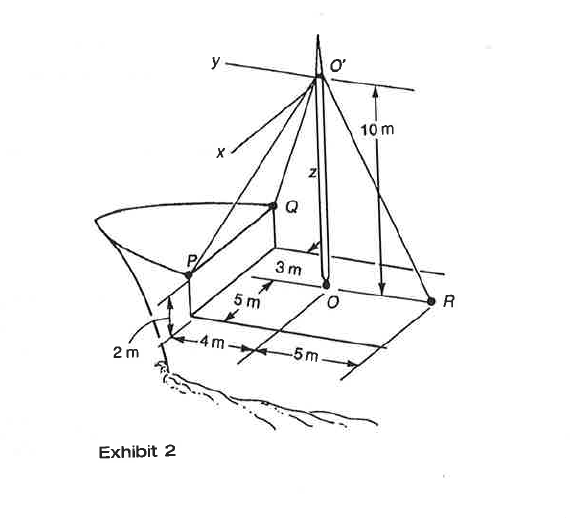
\includegraphics[scale=.35]{lecture1_fig1.png}
 	\small
 	\begin{enumerate}
 		\item Determine the lengths of the guylines O'P and O'Q and the angle between them.\\
 		
 		\item Suppose the guy line O'P has a tension of 800N. What is the moment from this force about O?
 		
 	\end{enumerate}
 	\end{multicols}
 	 \vspace{20mm}
  
}

\frame{
	\frametitle{\sectiontitleV}	
	
	Example 1 (cont.): \\
		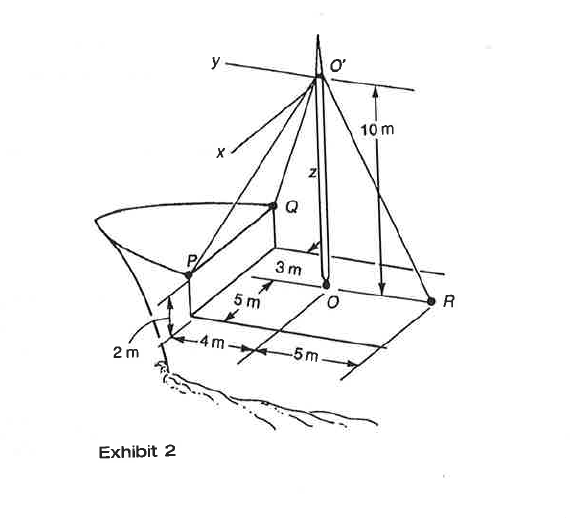
\includegraphics[scale=.35]{lecture1_fig1.png}
		\small


	\vspace{20mm}
	
}

\frame{
	\frametitle{\sectiontitleV}	
	
	Example 1 (cont.): \\
	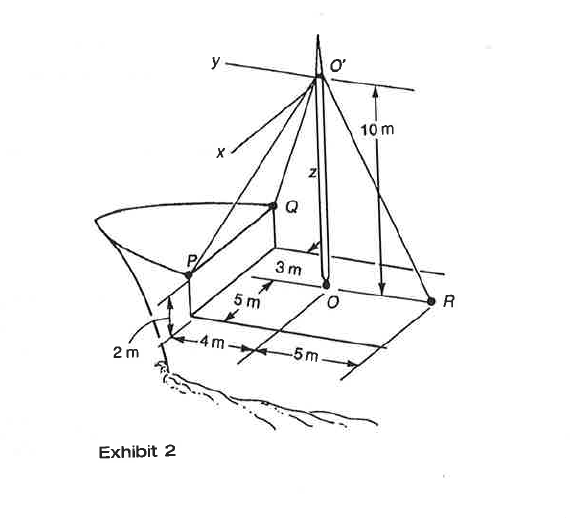
\includegraphics[scale=.35]{lecture1_fig1.png}
	\small
	
	
	\vspace{20mm}
	
}
 
 
\frame{
	\frametitle{\sectiontitleV}	
	
	Example 2: \\
	\begin{multicols}{2}
		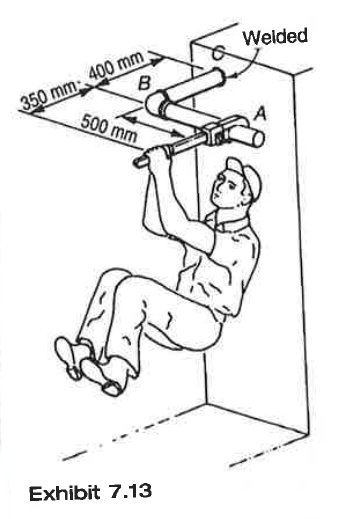
\includegraphics[scale=.4]{lecture1_fig2_cropped.png}
		\small
		
		The plumber in Exhibit 7.13 exerts a vertical downward force of 1 kN on the wrench handle. The moment about C of this force has a magnitude of: 
		\begin{enumerate}
			\item 500 N-m
			\item 750 N-m
			\item 900 N-m
			\item 1250 N-m
		\end{enumerate}
	\end{multicols}
	\vspace{20mm}
	
}

\frame{
	\frametitle{\sectiontitleV}	
	
	Example 1 (cont.): \\
	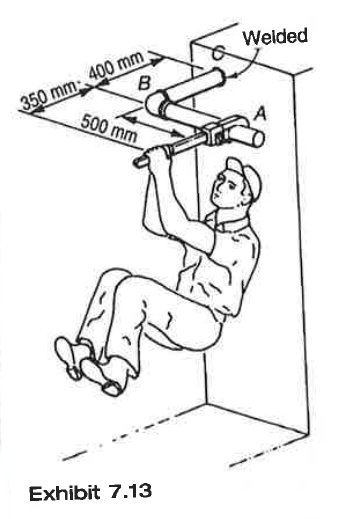
\includegraphics[scale=.4]{lecture1_fig2_cropped.png}
	\small
	
	
	\vspace{20mm}
	
}
 
  
\end{document}
